\documentclass[conf]{new-aiaa} % Use [journal] for AIAA journal style

%\usepackage[utf8]{inputenc}

%graphics packages
\usepackage[]{graphicx}
\graphicspath{{./figures/}}

% ------------------ tikz ------------
%%tikz
\RequirePackage{pgf,tikz, luatex85}
\usepackage{pgfplots}
\usepackage{booktabs} % in your preamble
\pgfplotsset{compat=newest}
\usetikzlibrary{arrows.meta}
\usetikzlibrary{arrows}
\usetikzlibrary{shapes.geometric}
\usetikzlibrary{shapes.misc}
\usetikzlibrary{backgrounds}
\usetikzlibrary{bending}
\usetikzlibrary{shadows}
\usetikzlibrary{patterns}
\usetikzlibrary{patterns.meta}
\usetikzlibrary{intersections}
\usepgfplotslibrary{patchplots}
\usepgfplotslibrary{fillbetween}
\usepgfplotslibrary{groupplots}
\usepgfplotslibrary{polar}
\usepgfplotslibrary{smithchart}
\usepgfplotslibrary{statistics}
\usepgfplotslibrary{dateplot}
\usepgfplotslibrary{ternary}


\pgfplotsset{%
	layers/standard/.define layer set={%
		background,axis background,axis grid,axis ticks,axis lines,axis tick labels,pre main,main,axis descriptions,axis foreground%
	}{grid style= {/pgfplots/on layer=axis grid},%
		tick style= {/pgfplots/on layer=axis ticks},%
		axis line style= {/pgfplots/on layer=axis lines},%
		label style= {/pgfplots/on layer=axis descriptions},%
		legend style= {/pgfplots/on layer=axis descriptions},%
		title style= {/pgfplots/on layer=axis descriptions},%
		colorbar style= {/pgfplots/on layer=axis descriptions},%
		ticklabel style= {/pgfplots/on layer=axis tick labels},%
		axis background@ style={/pgfplots/on layer=axis background},%
		3d box foreground style={/pgfplots/on layer=axis foreground},%
	},
}
% new style at automates partial ellipse
\tikzset{
    partial ellipse/.style args={#1:#2:#3}{
        insert path={+ (#1:#3) arc (#1:#2:#3)}
    }
}

\usepackage{caption}
\usepackage{subcaption}
\usepackage{placeins}
\usepackage{wrapfig}
\usepackage{url}
\usepackage{hyperref}

%tables
\usepackage{array}
\newcommand{\PreserveBackslash}[1]{\let\temp=\\#1\let\\=\temp}
\newcolumntype{C}[1]{>{\PreserveBackslash\centering}m{#1}}
\newcolumntype{R}[1]{>{\PreserveBackslash\raggedleft}m{#1}}
\newcolumntype{L}[1]{>{\PreserveBackslash\raggedright}m{#1}}

%mathpackages
\usepackage{amsmath}
%\usepackage{siunitx}
%\usepackage{mathrsfs}
%\newcommand{\vect}{\overset{\rightharpoonup}}
%decrease overset height
% \makeatletter
% \newcommand{\oset}[3][0.25ex]{%
% 	\mathrel{\mathop{#3}\limits^{
% 			\vbox to#1{\kern-0.5\ex@
% 				\hbox{$\scriptstyle#2$}\vss}}}}
% \makeatother

%%Vector arrow over variable
%\newcommand{\vect}[1]{%
%	\oset{\rightharpoonup}{#1}}

\RequirePackage{bm}
\newcommand{\vect}[1]{\bm{#1}}

\newcommand{\mat}[1]{%
	\mathbf{#1}}
\usepackage{nicefrac}
\usepackage{cancel}

%referencing packages
\usepackage[]{cleveref}
\usepackage{hyperref}
\usepackage{float}
\usepackage{placeins}

% ---------- colors -------------
\RequirePackage{xcolor}
\definecolor{navy}{HTML}{002E5D}
\definecolor{royal}{HTML}{005CAB}	% royal that matches BYU Engineering logo
\definecolor{darkgray}{HTML}{141414}
\definecolor{mediumgray}{HTML}{666666}	% medium gray definition from A. Ning
\definecolor{black}{HTML}{111111}
\definecolor{primary}{HTML}{005CAB}
\definecolor{secondary}{HTML}{c05367}
\definecolor{tertiary}{HTML}{8fa651}
\definecolor{plotsgray}{HTML}{808080}


% -------------- easy coloring of things ----------------
\newcommand{\navy}[1]{{\color{navy}#1}}
\newcommand{\primary}[1]{{\color{primary}#1}}
\newcommand{\secondary}[1]{{\color{secondary}#1}}
\newcommand{\tertiary}[1]{{\color{tertiary}#1}}
\newcommand{\gray}[1]{{\color{gray}#1}}

% Allow same footnotes
\newcommand*\samethanks[1][\value{footnote}]{\footnotemark[#1]}

% make \noindent where easier
\newcommand{\where}{\noindent where }
 % your preamble.tex file with packages

\begin{document}
\sloppy % helps reduce overfull hboxes

\title{Lab 1: A Tensile Test on 1018 Steel and 6061 Aluminum}
\author{Nathan R. Lehnhof\footnote{Mechanical Engineering}}
\affil{BYU Provo, UT}
\date{\today}
\maketitle

% ======================================================
\begin{abstract}
Lab 1 determines the value of the ultimate strength, yield strength, and the modulus of elasticity of Steel 1018 (cold rolled) and 6061 Aluminum by performing tensile tests.
Ultimate strength is the maximum stress a material can withstand before noticable necking.
It's the peak point on the engineering stress-strain curve.
Yield stress is the stress at which the material begins to noticibly plastically deform, generally at 0.002 strain.
Young's Modulus of Elasticity is the measure of a material's stiffness, being the slope of the elastic region of the stress-strain graph.
\end{abstract}

% ======================================================
\section{Methods}
To perform the tensile test, Steel 1018 and 6061 Aluminum "dog-bones" were placed in the tensile tester.
The "dog-bones" had a diameter of 0.3 inches (0.0762 mm) and a gauge length of 2.3 inches (0.5842 mm).
The tensile tester than gradually increases the tensile force experienced by the specimens, recording the force and the length of the specimen.
The data was returned as an excel file.
Because the tensile tester takes data so quickly, the last few data points of the file are after fracture, so those are manually removed.
Similarly, the tensile tester secures the samples with clamps.
That clamping produces an initial compressive force.
Those points are also manually removed post-process.

\begin{align}
    \sigma &= \frac{F}{A} \label{stress}
    && \text{Stress (MPa)} \\[6pt]
    \epsilon &= \frac{\delta l}{l_0} \label{strain} 
    && \text{Strain}
\end{align}

Since we need stress and strain, we use \autoref{stress} and \autoref{strain}.
From the Force (N) and diameter (mm), we find stress by dividing the force by the initial cross-sectional area.
To find strain, we first need to normalize our length, taking the first length as 0.0.
Then, we can use \autoref{strain} to find strain.
We then graph stress-strain for both Steel 1018 and 6061 Aluminum.
From these graphs, we can determine young's modulus, yield stress, and ultimate tensile stress as shown in the following tables.

\begin{figure}[h!]
\centering

\begin{minipage}{0.48\textwidth}
    \centering
    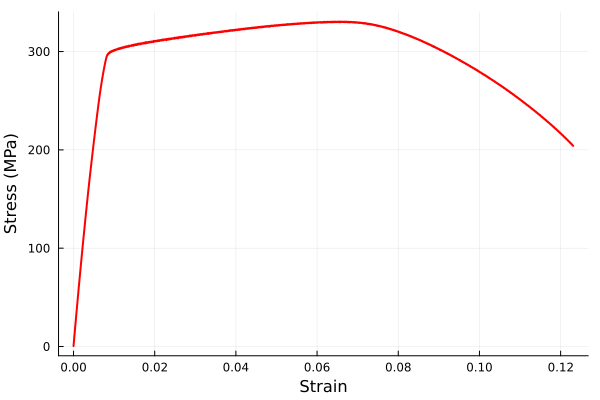
\includegraphics[width=\linewidth]{aluminum_plot.png}
    \caption{Stress-strain curve for 6061 Aluminum.}
    \label{fig:aluminum}
    \vspace{2em}
    \renewcommand{\arraystretch}{1.3}
    \begin{tabular}{lcc}
    \toprule
    \textbf{6061 Aluminum} & Expected & Actual \\
    \midrule
    Ultimate Strength (MPa) & 330 & 310 \\ 
    Yield Strength (MPa)    & 290 & 276 \\ 
    Modulus $E$ (GPa)       & 69  & 54 \\ 
    \bottomrule
    \end{tabular}
    \captionof{table}{Mechanical properties of 6061 Aluminum.}
    \label{tab:aluminum}
\end{minipage}
\hfill
\begin{minipage}{0.48\textwidth}
    \centering
    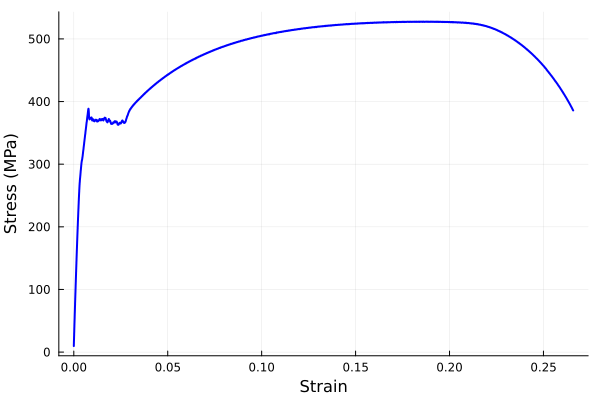
\includegraphics[width=\linewidth]{steel_plot.png}
    \caption{Stress-strain curve for Steel 1018 Cold-Rolled.}
    \label{fig:steel}
    \vspace{2em}
    \renewcommand{\arraystretch}{1.3}
    \begin{tabular}{lcc}
    \toprule
    \textbf{Steel 1018} & Expected & Actual \\
    \midrule
    Ultimate Strength (MPa) & 527 & 440 \\ 
    Yield Strength (MPa)    & 380 & 370 \\ 
    Modulus $E$ (GPa)       & 217 & 200 \\ 
    \bottomrule
    \end{tabular}
    \captionof{table}{Mechanical properties of Steel 1018.}
    \label{tab:steel}
\end{minipage}

\end{figure}

% ======================================================
\section{Conclusion}
We are more interested in the stress-strain curve than a force-displacement curve because stress and strain allows us to calculate yield stress, ultimate tensile stress, and young's modulus.
A force and displacement graph only works for the specific geometry of the dog-bone.
The stress-strain graph reflects the material properties that can be used with a range of geometries.
The values calculated from the stress-strain graph can be used universally with that material.

True stress uses the instantaneous area.
True strain uses the instantaneous change in length.
While true stress/strain reflects the more accurate properties, true tests are more costly.
Engineering stress and strain is sufficient for engineering purposes.
A tensile test would be necessary for the following: Space Shuttle, Suspension Bridge hangers or Truss Members, Lifting Equiment, Fasteners under Tension, Cables for Elevators/Cranes.

Some potential sources of error include machine calibration (unlikely), human error in placing/aligning dog-bones (more likely since it would change the gauge length), and the machining of the dog-bones (introduce heat/properties into the material).
Another important point is that this is only one sample.
As the number of samples increases, the accuracy of our values will increase.
We can most likely reduce error by increasing the number of tests and increasing consistency in machining the dog-bones.

% \section{References and Resources}

% \nocite{*}
% \bibliographystyle{new-aiaa}
% \bibliography{references}

\end{document}
